\chapter{Decision Making with Data Analytics Using R}

In a world overflowing with data, decision-making increasingly depends on how effectively we analyze and interpret this data. For fields like climate and agriculture, where choices directly impact communities and ecosystems, transforming raw data into actionable knowledge is crucial. However, successful decisions require more than just numbers—they demand clarity, context, and an awareness of potential biases to ensure fairness and trust.

This chapter explores how R-based data analytics can power better decisions by turning complex climate and agricultural data into clear, actionable insights. You will see practical examples and R code illustrating key steps in the decision-making process.

\section{The Role of Data Analytics in Decision Making}

\subsection*{What Data Analytics Brings to the Table}
Data analytics reveals hidden patterns and relationships in large datasets that would otherwise be invisible. In climate and agriculture, it can:
\begin{itemize}
    \item Forecast extreme weather events like droughts or floods, enabling preparedness
    \item Identify factors affecting crop yields for improved farming practices
    \item Optimize resource use, such as water and fertilizers
    \item Help policymakers allocate resources effectively and plan interventions
\end{itemize}

\subsection*{From Raw Data to Informed Decisions}
Raw data alone is often overwhelming and difficult to interpret. The analytical journey converts this raw data into:
\begin{itemize}
    \item \textbf{Descriptive insights}: What has happened? (e.g., trends in rainfall over 10 years)
    \item \textbf{Diagnostic insights}: Why did it happen? (e.g., correlation between temperature rise and crop failure)
    \item \textbf{Predictive insights}: What might happen next? (e.g., forecasting seasonal precipitation)
    \item \textbf{Prescriptive insights}: What actions should be taken? (e.g., recommending drought-tolerant crop varieties)
\end{itemize}

Moving through these stages helps shift decision-making from reactive responses to proactive planning.

\section{Communicating Insights Effectively}

\subsection*{The Challenge}
Data scientists often use technical jargon and complex visuals, which may confuse stakeholders like farmers, local officials, or policymakers.

\subsection*{Principles for Clear Communication}
\begin{itemize}
    \item \textbf{Simplicity}: Use straightforward language and avoid jargon
    \item \textbf{Relevance}: Focus insights on stakeholder concerns and decisions
    \item \textbf{Visual clarity}: Use simple, clear charts and infographics
    \item \textbf{Actionability}: Always suggest next steps or decisions based on insights
\end{itemize}

\subsection*{R Example: Communicating Crop Production Trends in Hilly Regions}

Suppose you have analyzed agricultural production data and want to communicate the yearly trends of top crops in hilly regions. Instead of presenting raw data tables, a clear line plot can effectively show these trends.

\begin{verbatim}
# Summarize yearly production for top crops

top_crops_list <- head(top_crops$Crop, 5)  # top 5 crops
yearly_trends <- merged_data %>%
  filter(Crop %in% top_crops_list) %>%
  group_by(Year, Crop) %>%
  summarise(
    Yearly_Production = sum(Production, na.rm = TRUE))

# Plot
ggplot(yearly_trends, aes(x = Year, y = Yearly_Production, color = Crop)) +
  geom_line(linewidth = 1) +
  labs(title = "Yearly Production Trends for Top Crops in Hilly Regions",
       x = "Year",
       y = "Production") +
  theme_minimal()
\end{verbatim}

% Figure here-----------------------------
\begin{figure}[h]
\centering
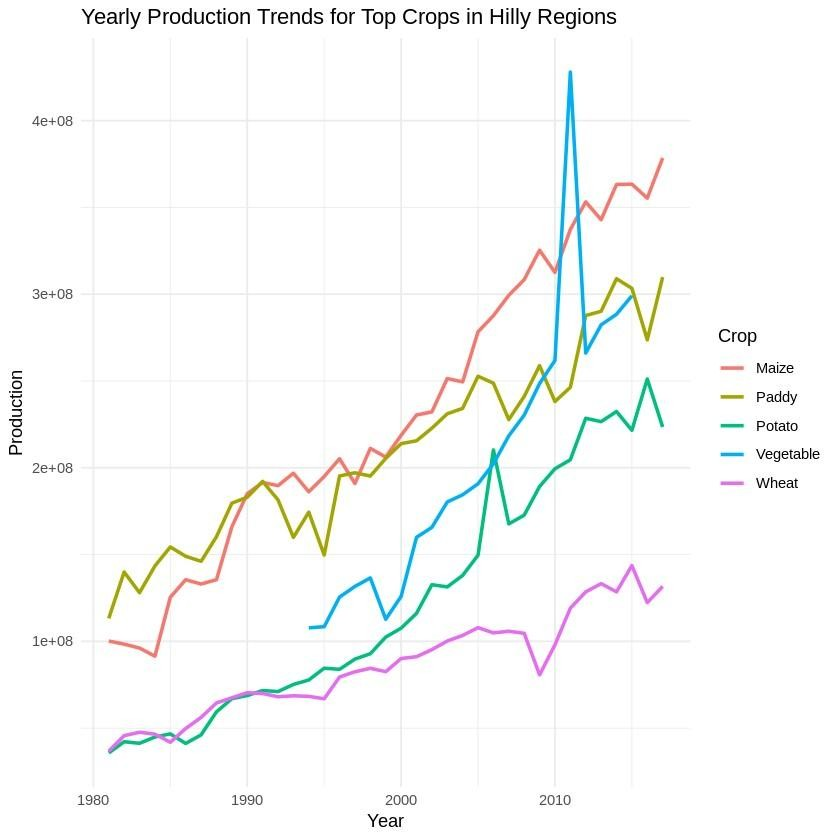
\includegraphics[width=0.5\textwidth]{figures/top5_agri.jpg}
\caption{Yearly Production Trends for Top Crops in Hilly Regions}
\end{figure}

\subsection*{What the Crop Production Graph Tells Us?}
This graph shows us how many different main crops like Maize, Paddy, Potatoes, Vegetables, and Wheat are grown in hilly areas each year.\\

\textbf{What We See:}
\begin{itemize}
    \item Maize and Paddy are the biggest crops. They produce the most food, and Maize has really shot up in recent years!
    \item Potatoes and vegetables are also growing a lot. People are growing more and more of these.
    \item Wheat is growing too, but not as much as the other main crops in hilly region.
\end{itemize}

\textbf{Why This Matters (and What Decisions We Can Make):}
\begin{itemize}
    \item \textbf{Support the Winners}: Since Maize and Paddy are doing so well, we should keep helping farmers grow more of them. Maybe give them better seeds or help with watering systems.
    \item \textbf{Check on Wheat}: Wheat isn't growing as fast. We might need to look into why. Is the soil not good? Is the weather changing? Maybe we should focus on other crops that do better here, or find special wheat that likes hilly areas.
    \item \textbf{Help Farmers Try New Things}: Encourage farmers to plant more Potatoes and Vegetables if they can, because these crops seem to be in high demand and can earn farmers more money.
\end{itemize}

\section{Detecting Bias and Ensuring Ethical Decision Making}

\subsection*{Understanding Bias in Climate Data}

Bias means something in the data is unfair or misleading. It can cause wrong conclusions and lead to poor decisions. It can distort the truth and lead to unfair or ineffective decisions. Common sources include:

\begin{itemize}
    \item \textbf{Sampling Bias}: We have more data from certain places or times, making our view incomplete (like only hearing from cities, not rural areas).
    \item \textbf{Measurement Bias}: Our tools consistently give incorrect readings (like a rain gauge always showing less rain than there actually was).
    \item \textbf{Analyst Bias}: Our personal beliefs accidentally shape how we see and explain the data.
    \item \textbf{Algorithmic Bias}: Our computer programs learn bad habits from skewed data and then make biased predictions themselves.
\end{itemize}

\subsection*{Why It Matters}
Imagine we're trying to figure out how weather affects everyone in a region. If most of our weather data only comes from big cities, but we forget to collect enough from the rural areas where people are farming every day, that's a problem!

This leads to serious problems:

\begin{itemize}
    \item \textbf{Wrong decisions}: Policies may not help farmers facing droughts or floods.
    \item \textbf{Missed warnings}: A remote village might suffer a drought we didn’t see coming.
    \item \textbf{Wasted resources}: Efforts go to the wrong places, ignoring where help is truly needed.
    \item \textbf{Unfair impact}: Some communities always benefit, while others are left out.
\end{itemize}

\subsection*{R Example: Detecting Sampling Bias in District-Level Climate Data}

If some districts have far fewer records, this indicates sampling bias that should be addressed to avoid misleading conclusions. Check if data is evenly distributed across districts:

\begin{verbatim}
district_counts <- df_climate %>%
  group_by(District) %>%
  summarise(Record_Count = n()) %>%
  arrange(desc(Record_Count))

# View the counts
print(district_counts)

# Set plot size (width x height in inches)
options(repr.plot.width = 12, repr.plot.height = 6)

# Plot the distribution
ggplot(district_counts, aes(x = reorder(District, -Record_Count), 
y = Record_Count)) +
  geom_bar(stat = "identity", fill = "steelblue") +
  labs(title = "Number of Climate Records per District",
       x = "District",
       y = "Record Count") +
  theme(axis.text.x = element_text(angle = 45, hjust = 1))
\end{verbatim}

% Figure here-----------------------------
\begin{figure}[h]
\centering
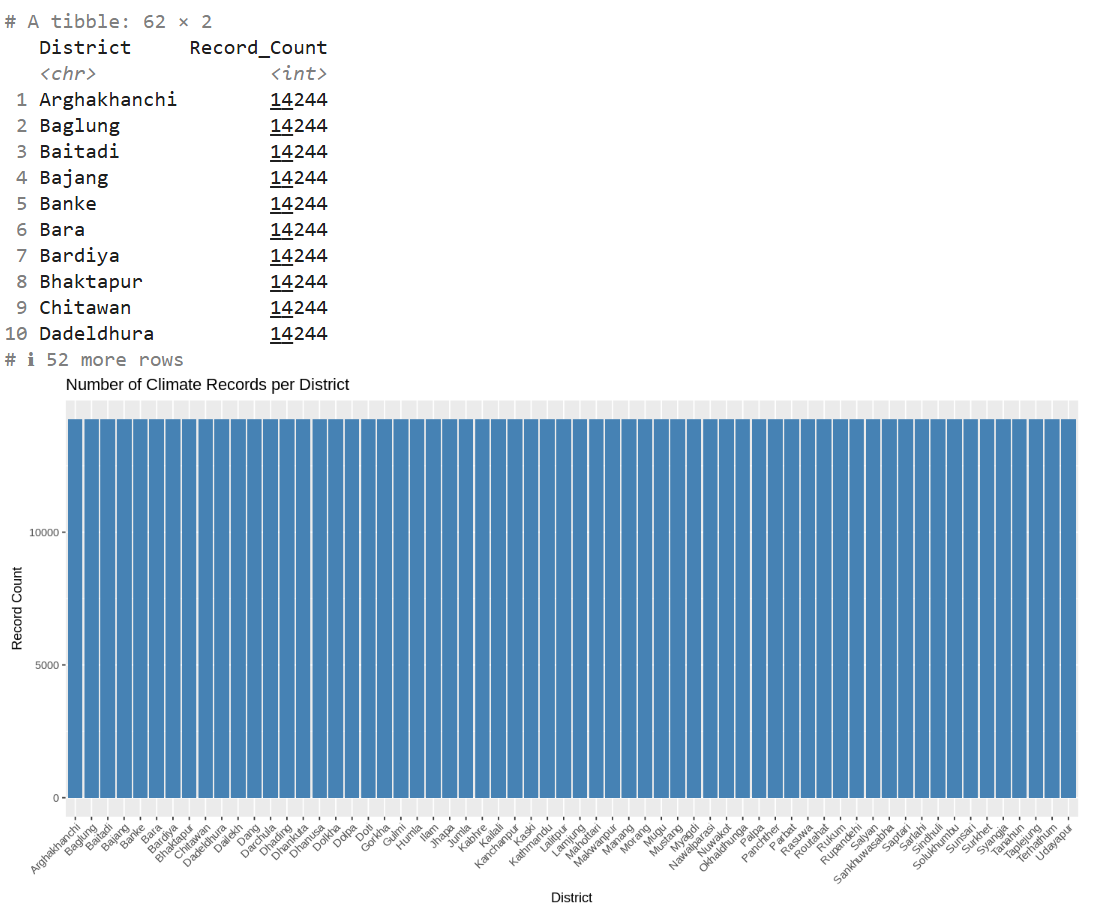
\includegraphics[width=0.6\textwidth]{figures/dist_count.png}
\caption{Number of Climate Records per District}
\end{figure}

The above plot displays the distribution of data counts across the 62 districts included in the dataset. However, it is important to note that data is available for only 62 out of the 77 total districts, meaning 15 districts are not represented.

\subsection*{Monitoring Temporal Bias}

Check if data collection is balanced across months:

\begin{verbatim}
# Count records per month
month_counts <- df_climate %>%
  group_by(Month_Label) %>%
  summarise(Count = n())

# Plot counts by month
ggplot(month_counts, aes(x = Month_Label, y = Count)) +
  geom_bar(stat = "identity", fill = "steelblue") +
  labs(title = "Monthly Distribution of Climate Data Records",
       x = "Month",
       y = "Number of Records") +
  theme_minimal()
\end{verbatim}

% Figure here-----------------------------
\begin{figure}[h]
\centering
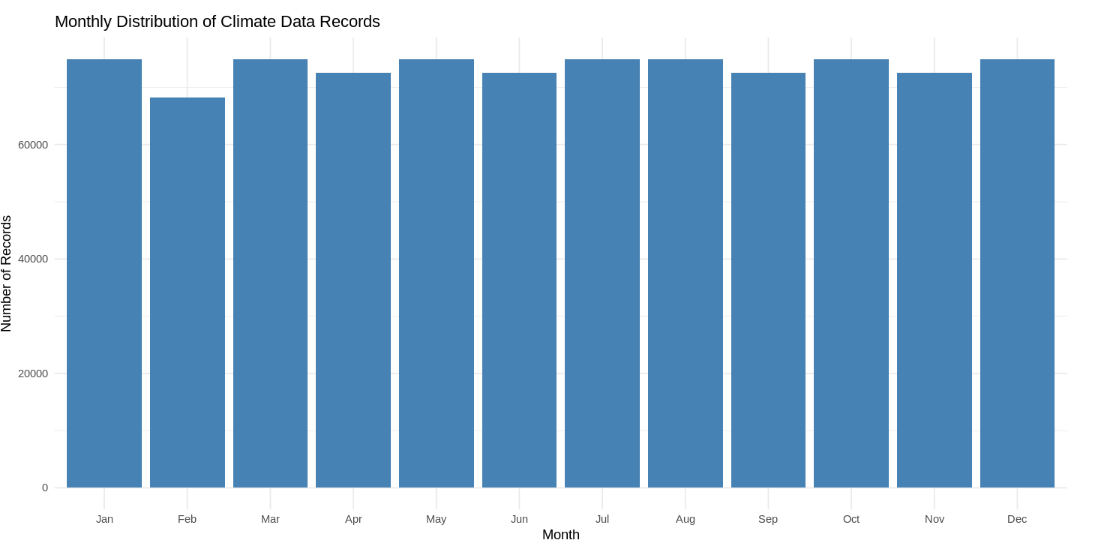
\includegraphics[width=0.5\textwidth]{figures/month_count.png}
\caption{Monthly Distribution of Climate Data Records}
\end{figure}

\section*{Summary}
\begin{itemize}
    \item Data analytics using R turns raw climate and agricultural data into clear, actionable decisions.
    \item Communicating results in simple, relevant, and visual ways empowers decision-makers.
    \item Detecting and correcting bias improves fairness and effectiveness.
    \item Ethical awareness ensures transparency, accountability, and respect for all stakeholders.
\end{itemize}
